
{
  \renewcommand{\sectionsubtitle}{How a node lives, reproduces, mutates, and dies}
  \section{The system}
}


{
\setbeamerfont{itemize/enumerate body}{size=\small} % template pins lists to \normalsize
\begin{frame}{System at a glance: one autonomous node}
  \small
  \begin{columns}[T, onlytextwidth]
    \begin{column}{0.46\textwidth}
      A node is one process running on a leased SporeStack (a Bitcoin-native marketplace) VPS with:
      \begin{itemize}
        \item \textbf{Bitcoin wallet} --- pays its own bills.
        \item \textbf{Seedbox} --- serves Creative Commons content.
        \item \textbf{IPv8 overlay} --- gossips health telemetry to peers.
        \item \textbf{Decision logic} --- the core actions.
      \end{itemize}

      \textcolor{tud Orange}{No central authority:} bootstraping genesis is the only human action. afterwards the fleet self-governs and no node has authority.
    \end{column}
    \begin{column}{0.5\textwidth}
      \centering
      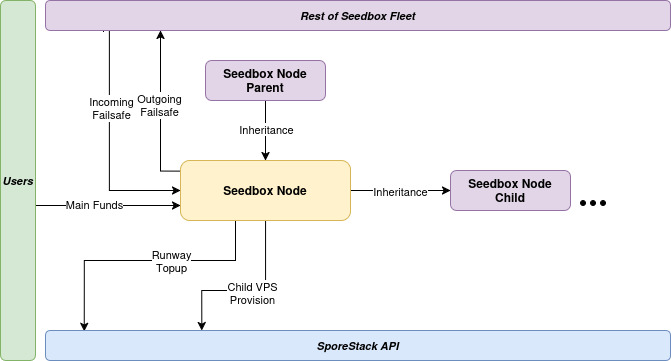
\includegraphics[width=\linewidth]{figures/NodeArchitectureSeedBox.jpg}\\[0.5ex]
      {\footnotesize Arrows trace Bitcoin movements.}
    \end{column}
  \end{columns}
\end{frame}
}


{
\setbeamerfont{itemize/enumerate body}{size=\small} % template pins lists to \normalsize
\begin{frame}{The decision loop}
  \framesubtitle{The main control logic}
  \small
  \begin{columns}[T, onlytextwidth]
    \begin{column}{0.5\textwidth}
      \centering
      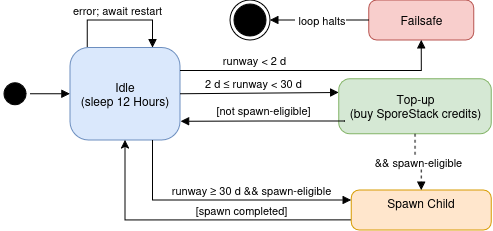
\includegraphics[width=\linewidth]{figures/decision_loop_statemachine.png}
    \end{column}
    \begin{column}{0.46\textwidth}
      Every 12 h, the node takes the first action whose guard passes:
      \begin{enumerate}
        \item \textbf{Failsafe} --- runway \textcolor{tud Orange}{< 2 days}
          \(\to\) sweep remaining funds to the richest peer.
        \item \textbf{Top-up} --- runway < 30 days \(\to\) buy VPS credits to cover another 30 days (\emph{does not end tick}).
        \item \textbf{Spawn} --- if eligible \(\to\) provision + fund a child.
        \item \textbf{Idle} --- wait for the next tick.
      \end{enumerate}

      \medskip
      \textbf{Identical code} runs in every node.
    \end{column}
  \end{columns}
\end{frame}
}


{
\setbeamerfont{itemize/enumerate body}{size=\small} % template pins lists to \normalsize
\begin{frame}{Reproduction mechanics}
  \small
  \begin{block}{Check post-spawn runway, not before}
    A node spawns only if its \textbf{post-spawn total runway}
    \(\geq 60\times(1+\text{caution})\) days \emph{and} its wallet can pay for the
    child's VPS. A node's \textbf{total runway} \(=\) VPS days \(+\) SporeStack credit
    \(+\) BTC.
  \end{block}

  \begin{itemize}
    \item The child starts with a \textbf{30-day} pre-paid VPS and inherits
      \textbf{40\%} of the Bitcoin remaining \emph{after} the parent covers the
      child's expenses.
    \item Actual Pipeline: mutate caution \(\to\) provision VPS \(\to\) fresh BTC wallet \(\to\) deploy code over SSH \(\to\) transfer inheritance.
  \end{itemize}
\end{frame}
}


{
  \setlength{\splitpos}{0.55\paperwidth} % colored pane left, title shifts right
  \leftfooterwhitetrue
  \begin{frame}{The heritable trait}
    \begin{columns}[T]
      \begin{textcolumn}
        \color{white}\large
        \textbf{Caution} --- the single trait under selection.

        \medskip
        \medskip
        \medskip
        \medskip
        \medskip
        \medskip
        Value \(c \in [0.35, 0.9]\), with the genesis node starting at \(c = 0.5\).
        Everything else is inherited.
      \end{textcolumn}
      \begin{textcolumn}
        \footnotesize
        It scales the spawn threshold \(60\times(1+c)\):

        \smallskip
        \begin{tabular}{cc}
          caution \(c\) & threshold \\
          0.35 & 81 days \\
          0.5  & 90 days \\
          0.9  & 114 days \\
        \end{tabular}

        \smallskip
        Low caution \(=\) spawn sooner \\  
        High caution \(=\) retain more 

        \smallskip
        Mutation Formula:\\
        \(c = c_{\text{parent}} + \mathcal{N}(0,0.05)
        + 0.2\,(0.5 - c_{\text{parent}})\) Gaussian drift with reversion to 0.5.

      \end{textcolumn}
    \end{columns}
  \end{frame}
}
\setlength{\splitpos}{0pt}\leftfooterwhitefalse % reset stateful split/footer
